\chapter{事前実験}
\label{prex}

本章では,~\ref{approach:problemofSshLowHoneypot}で述べた手法を実現するための事前実験を概説する.

\subsection{概要}
\label{prex:abst}
SSHの低対話型HoneypotであるCowrieはコマンドの実装数が少なく,Cowrie特有の異常な挙動が多く,本来実際のOSへの攻撃であれば取れるはずであった侵入ログが取れない問題がある.また,収集ログを分析する際に,これまで用いられてきた"危険なコマンド"としてインデックスを作り,それらを危険なコマンドとしてパターンマッチングする手法では,今後出現してくる様々なコマンドパターンなどに対応できない.\\
予備実験では,実装を施していない純正のCowrieとCowrieにBusyBoxに含まれるコマンドを実装した修正済みのCowrieの両方でコマンドログの収集を行うことで,実装を施していない純正のCowrieで収集した侵入ログとCowrieにBusyBoxに含まれるコマンドを実装した修正済みのCowrieで収集した侵入ログとでは,収集ログのパターンに変化があるのではないかと考えた.評価として収集した二つのログをSkip-gramモデルを用いてスコアリングし,どちらがより多くのコマンドログのパターンを収集できているのかを検証した.\\
その結果,より多くのコマンドパターンを取れたのがCowrieにBusyBoxに含まれるコマンドを実装した修正済みのCowrieであるという結果を出した.

\subsection{要素技術}
\label{prex:tech}
予備実験の要素技術に関しては第2章の要素技術で全て説明している.

\subsection{問題定義}
\label{prex:method}
侵入者に侵入先がSSHの低対話型Honeypotであると検知されてしまい,本来取れるはずの収集ログが収集できないため,本来実際のOSへの攻撃であれば取得できたはずの侵入ログが収集できない.

\subsection{予備実験の手法}
\label{prex:appr}
実装を施していない純正のCowrieに対して,これには実装されていないがShellには実装されているコマンドを実装した.

\subsection{実装}
\label{prex:impl}
純正のCowrieにBusyBoxに含まれるコマンドを実装し,またHoneypot特有の異常な挙動を修正した.予備実験の実装に関しては第6章の実装で全て説明している.

\subsection{評価}
\label{prex:eval}
実装を施していない純正のCowrieとCowrieにBusyBoxに含まれるコマンドを実装した修正済みのCowrieの両方で侵入ログの収集を行い,Word2vecのSkip-Gram Modelにより次のコマンドの予測,スコアリングを行い評価をした.スコアリングでは,あるコマンドが実行された時に次のコマンドの出やすさを予測したため,次に実行されるコマンドがスコアとして高い数値を出せばそのコマンドパターンがパターンとして存在しやすいもであるというものである.予備実験の評価に関しては第7章の評価で一部説明している.
本研究の評価と違う評価手法としては,モデル化を純正のHoneypotにBusyBoxに含まれるコマンドを実装したものしか行っていないため,実際のOSに近いログが取れたことが証明できておらず,比較する対象が少なかった.

\subsection{結果}
\label{prex:conc}
SSHの低対話型Honeypotの稼働期間は12/10\~2/1(54日間)で,収集できたものとしてコネクション数,パターン数,コマンド数を以下の図3に記す.

\begin{figure}[H]
    \centering
    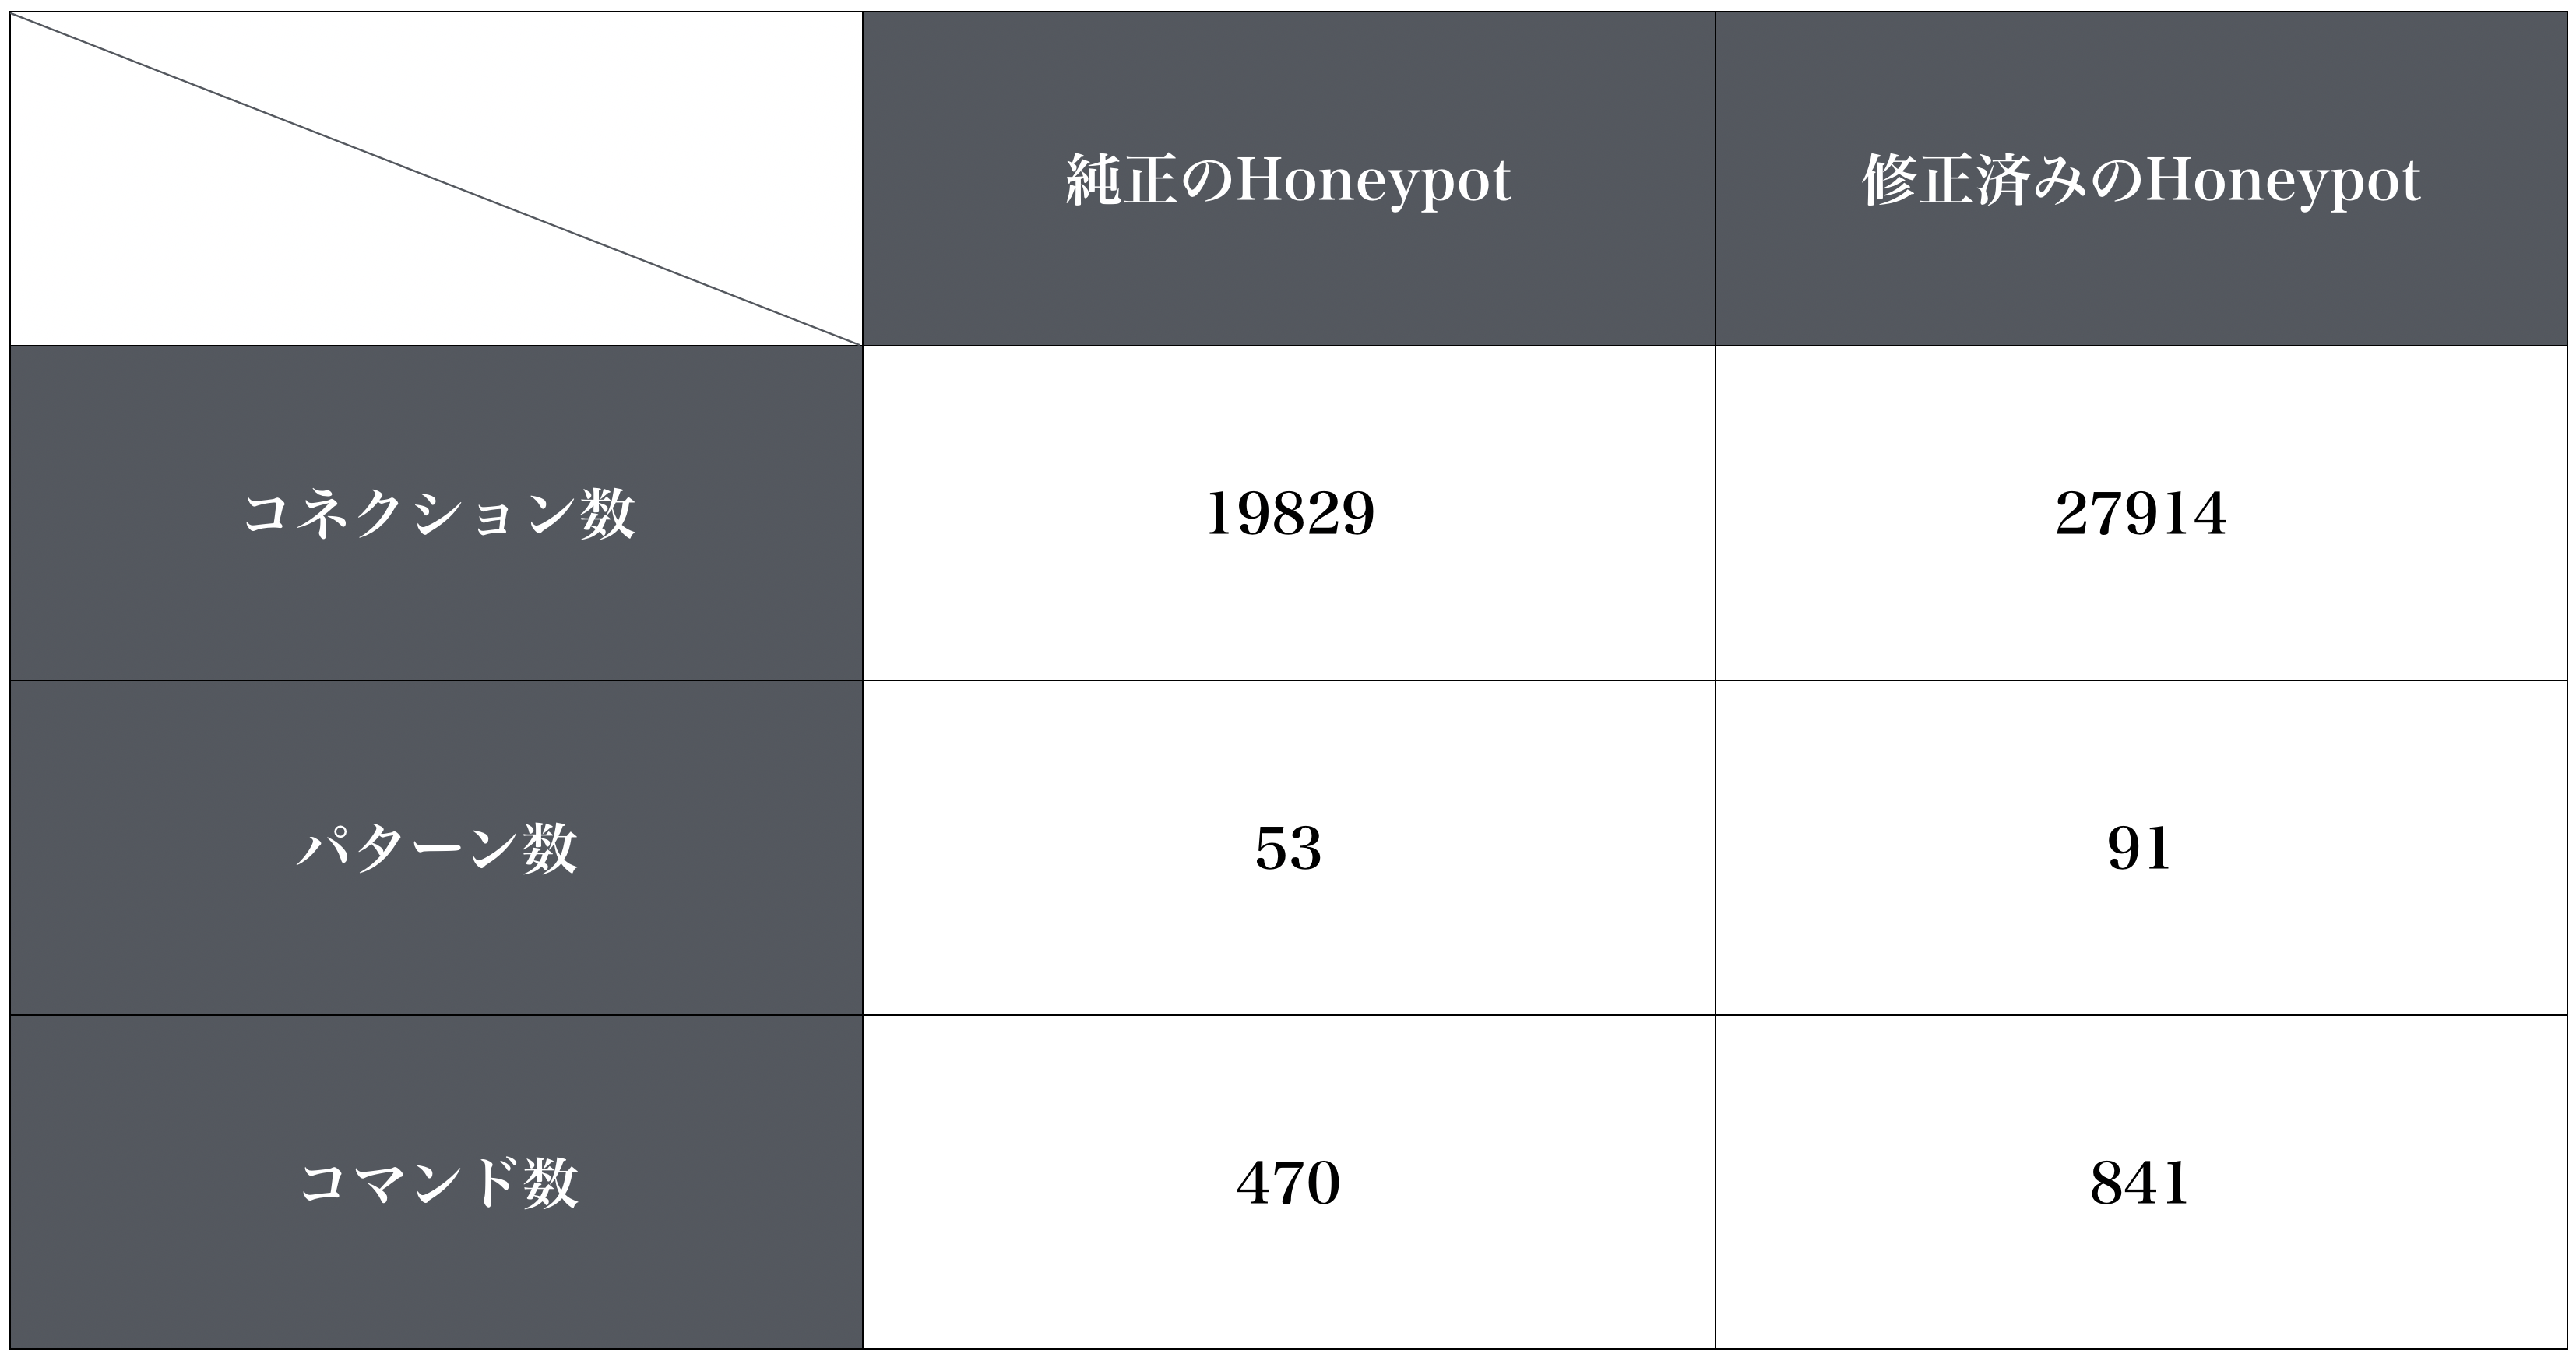
\includegraphics[width=1.0\textwidth]{figures/term.png}
    \caption{収集したSSHの低対話型Honeypotのデータ}
    \label{fig:evo}
\end{figure}

また,モデル化を行い純正のCowrieとCowrieにBusyBoxに含まれるコマンドを実装した修正済みのCowrieのスコアリングを行なった結果を以下の図4に記す.

\begin{figure}[H]
    \centering
    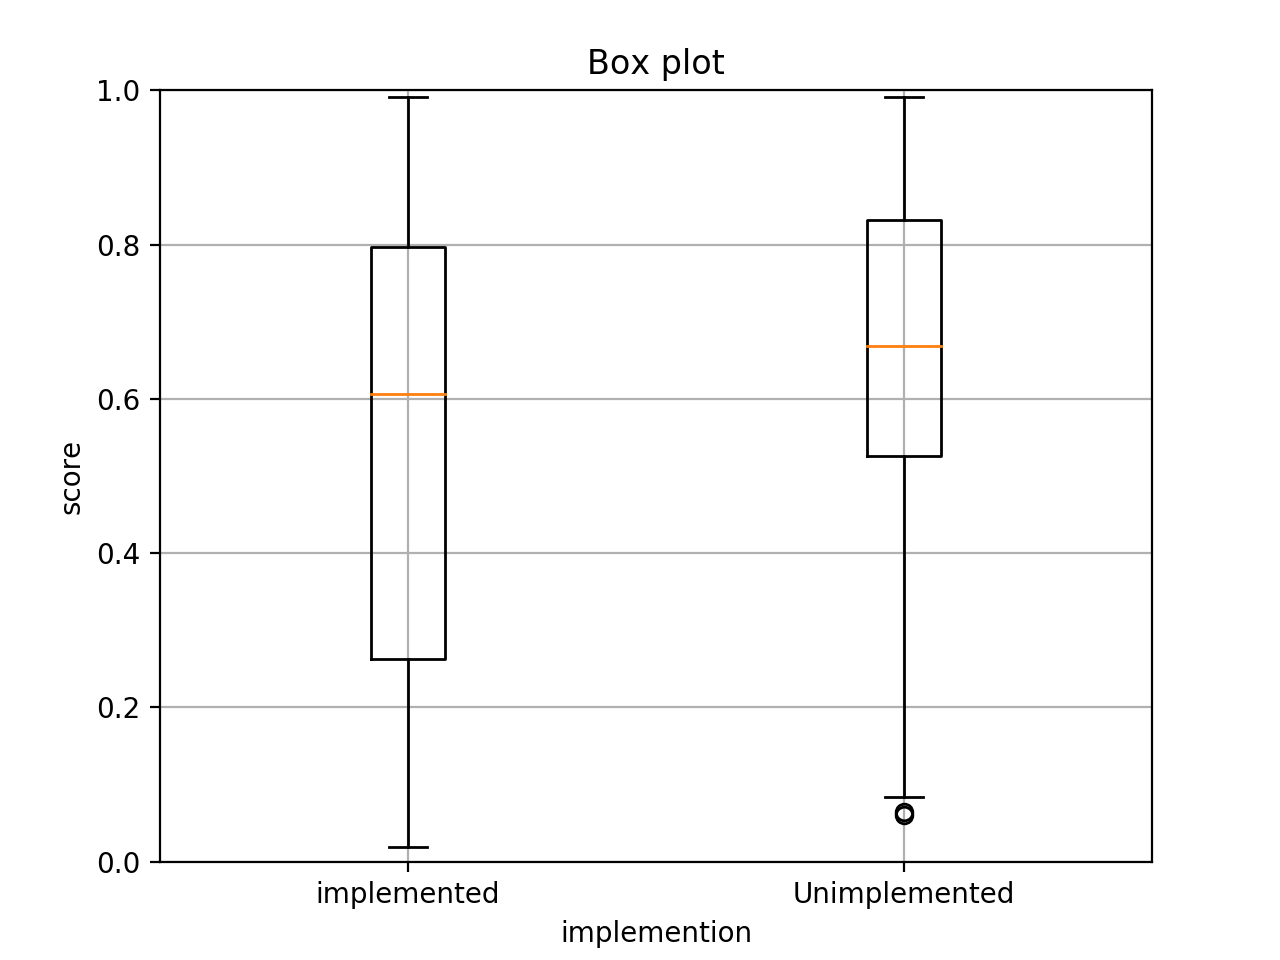
\includegraphics[width=1.0\textwidth]{figures/Figure_1.png}
    \caption{純正のCowrieと修正済みのCowrieのスコアリングによる比較}
    \label{fig:evo}
\end{figure}

本研究の予備実験では,Cowrieに実装されていないコマンドで悪意のある侵入者が使うようなコマンドを実装し,何の追加実装も施していないCowrieで取れた侵入者の実行コマンドログと ,追加実装を施したCowrieの侵入者の実行コマンドログを比較することで,追加実装を施したSSHのCowrieの方がコマンドパターンとして多く収集できることを示した.


%%% Local Variables:
%%% mode: japanese-latex
%%% TeX-master: "../bthesis"
%%% End: